\chapter{方法设计}
\label{chap:algorithm}

\section{棋盘规则}
超级皇后的棋盘继承国际象棋的规格,并且可以根据喜好扩大盘面($8\times8$,$12\times12$,$16\times16$等等)。在我们设计的API中,游戏开始时棋盘的大小可以任意自定义。受限于设备,AlphaZero框架的AI玩家只训练了$8\times8$棋盘(经典棋盘)。因此在本文中我们主要关心$8\times8$棋盘的结果。
超级皇后对战的规则也可以在我们设置的api中指定,如引言中所述,超级皇后走法规则可选三个规则:

(1)超级状态(super),拥有皇后和骑士的权限,可按此两种棋子落子规则任意移动;

(2)皇后状态(queen),可横竖对角线移动,不可越过移动直线上的对手;

(3)骑士状态,可走“日”字,即先向左(或右)走1格,再向上(或下)走2格;或先向左(或右)走2格,再向上(或下)走1格。

棋盘每个位置都具有四个状态值候选:$\{white:1, black:-1,empty:0,dead:99\}$,抛开初始位置(左上角与右下角),剩余位置的状态转换如下所示:
\begin{equation}
    \begin{aligned}
    empty &\stackrel{\mathrm{move}}{\longrightarrow} black \stackrel{\mathrm{leave}}{\longrightarrow} dead \\
    empty &\stackrel{\mathrm{move}}{\longrightarrow} white \stackrel{\mathrm{leave}}{\longrightarrow} dead 
    \end{aligned}
\end{equation}

依据信息暴露程度,超级皇后对战属于完美信息游戏(Perfect-Information Game)~\cite{binmore2007game}。对于完美信息游戏,可以用状态空间复杂度(State-Space Complexity)和博弈树复杂度(Game-Tree Complexity)对其难度进行衡量~\cite{allis1994searching,VANDENHERIK2002277}。
状态空间复杂度是指从初始状态开始,可以实现的所有符合规则的状态的集合总数,在实际情况中一般使用该数量的上界表示,例如在围棋中允许出现全白或全黑的极端情况。
博弈树复杂度表示所有不同游戏路径数目,常用合理估计的下界表示:$valids^{turn}$。 $valids$表示每回合平均合法移动数目,$turn$表示平均游戏长度~\cite{10.1007/BF00992697}。
类似于国际象棋与围棋,我们可以给出超级皇后对战的状态空间与博弈树复杂度(仅考虑$8\times8$棋盘),如表~\ref{table:complexity}。
% \begin{figure}[htb]
%     \centering
%     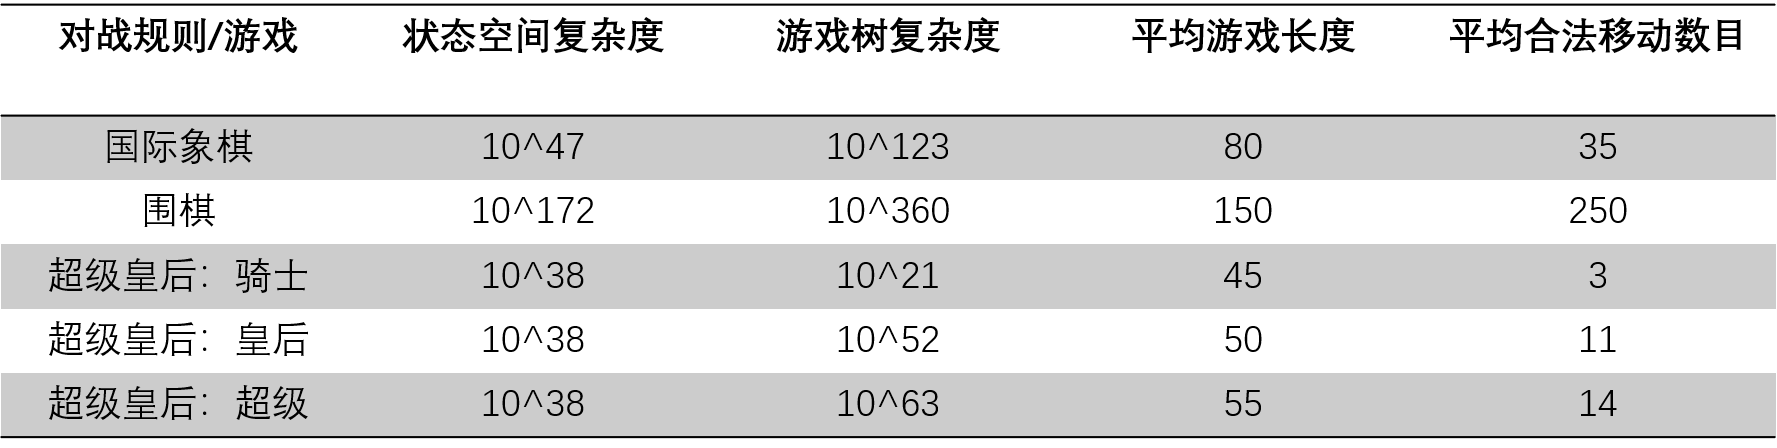
\includegraphics[width=1\textwidth]{complexity.png}
%     \caption[complexity]{%
%         超级皇后对战复杂度\cite{enwiki:complexity}%
%       }
%     \label{fig:complexity}
% \end{figure}
\begin{table}[htb]
  \centering
  \caption[complexity]{超级皇后对战游戏复杂度,国际象棋与围棋数据来自~\cite{enwiki:complexity}}
  \begin{tabular}{p{3cm}<{\centering} p{2cm}<{\centering} p{2cm}<{\centering} p{2cm}<{\centering} p{2cm}<{\centering}}
  \hline
  对战规则/游戏 & 状态空间复杂度 & 游戏树复杂度 & 平均游戏长度 & 平均合法移动数目 \\ \hline
  国际象棋 & $10^{47}$ & $10^{123}$&$80$ &$35$\\ 
      围棋 & $10^{172}$ & $10^{360}$&$150$ &$250$ \\ 
      超级皇后:骑士 & $10^{38}$ & $10^{21}$ &$45$ & $3$\\ 
      超级皇后:皇后 & $10^{38}$ & $10^{52}$ & $50$ & $11$\\ 
      超级皇后:超级 & $10^{38}$ & $10^{63}$ & $55$ & $14$\\ \hline
  \end{tabular}
  \label{table:complexity}
\end{table}

\begin{figure}[htb]
    \centering
    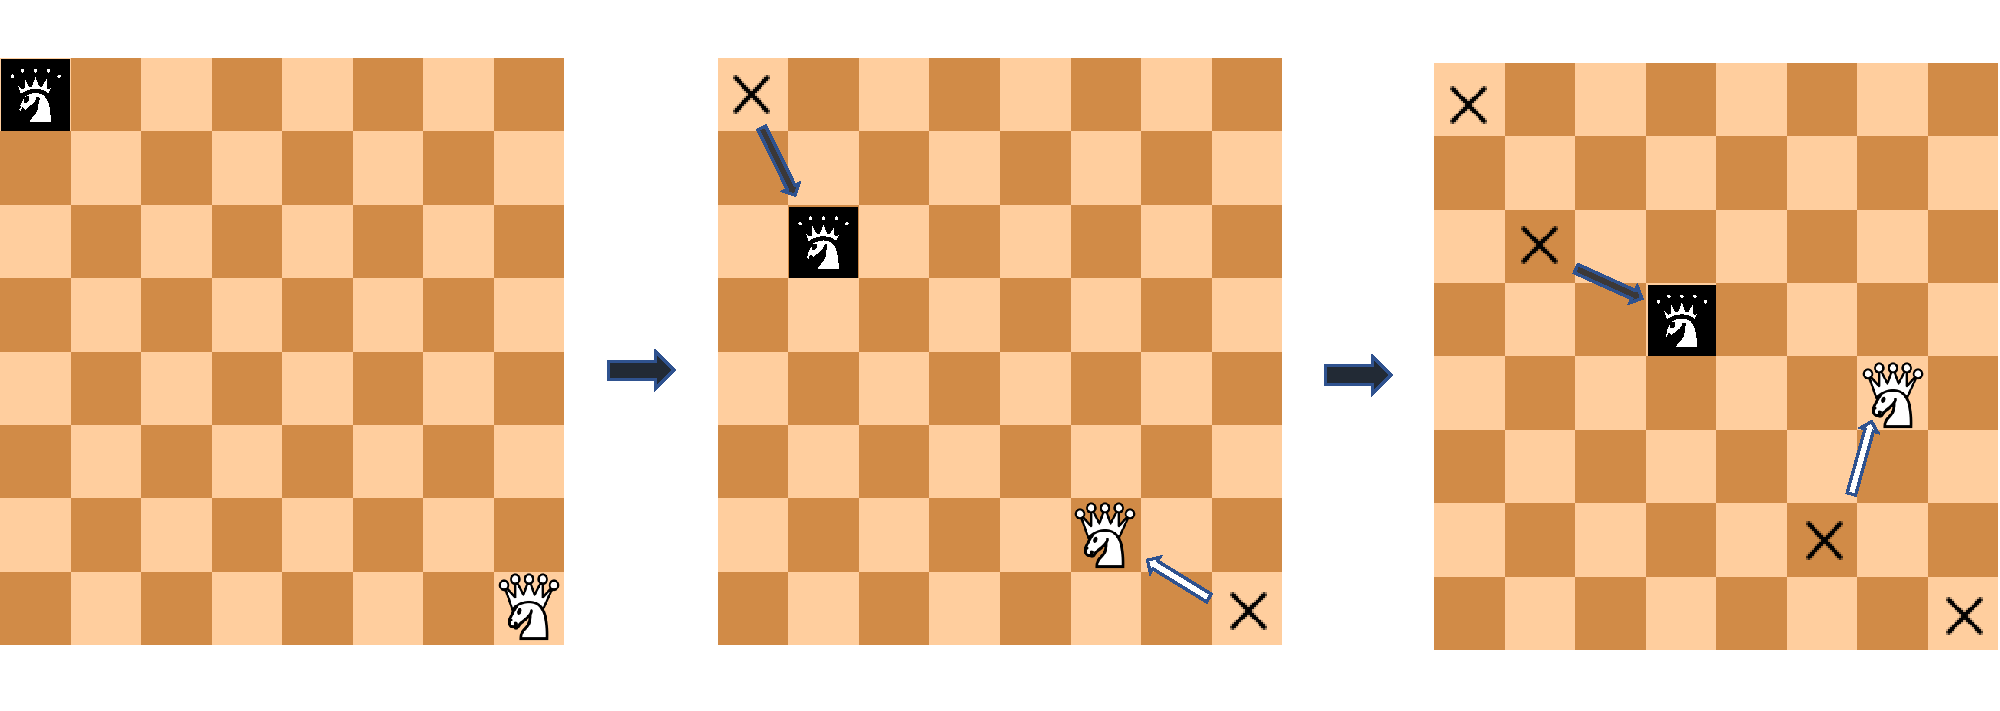
\includegraphics[width=0.8\textwidth]{knight.pdf}
    \caption[rules-knight]{%
        超级皇后对战游戏规则——骑士状态%
      }
    \label{fig:knight}
\end{figure}

\begin{figure}[htb]
    \centering
    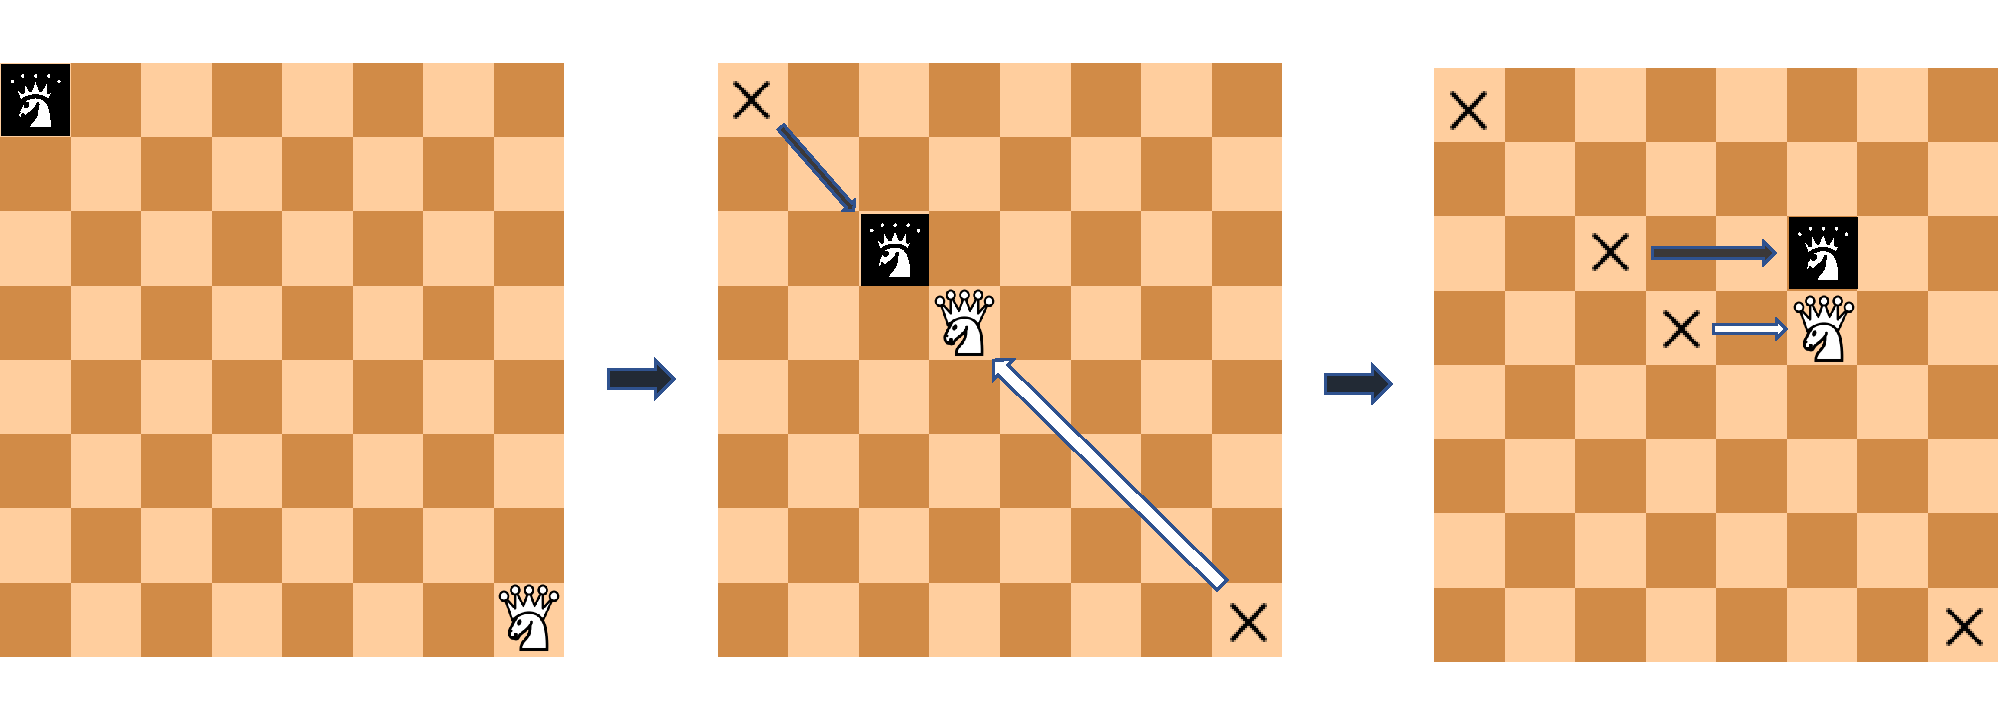
\includegraphics[width=0.8\textwidth]{queen.pdf}
    \caption[rules-queen]{%
        超级皇后对战游戏规则——皇后状态%
      }
    \label{fig:queen}
\end{figure}

\begin{figure}[htb]
    \centering
    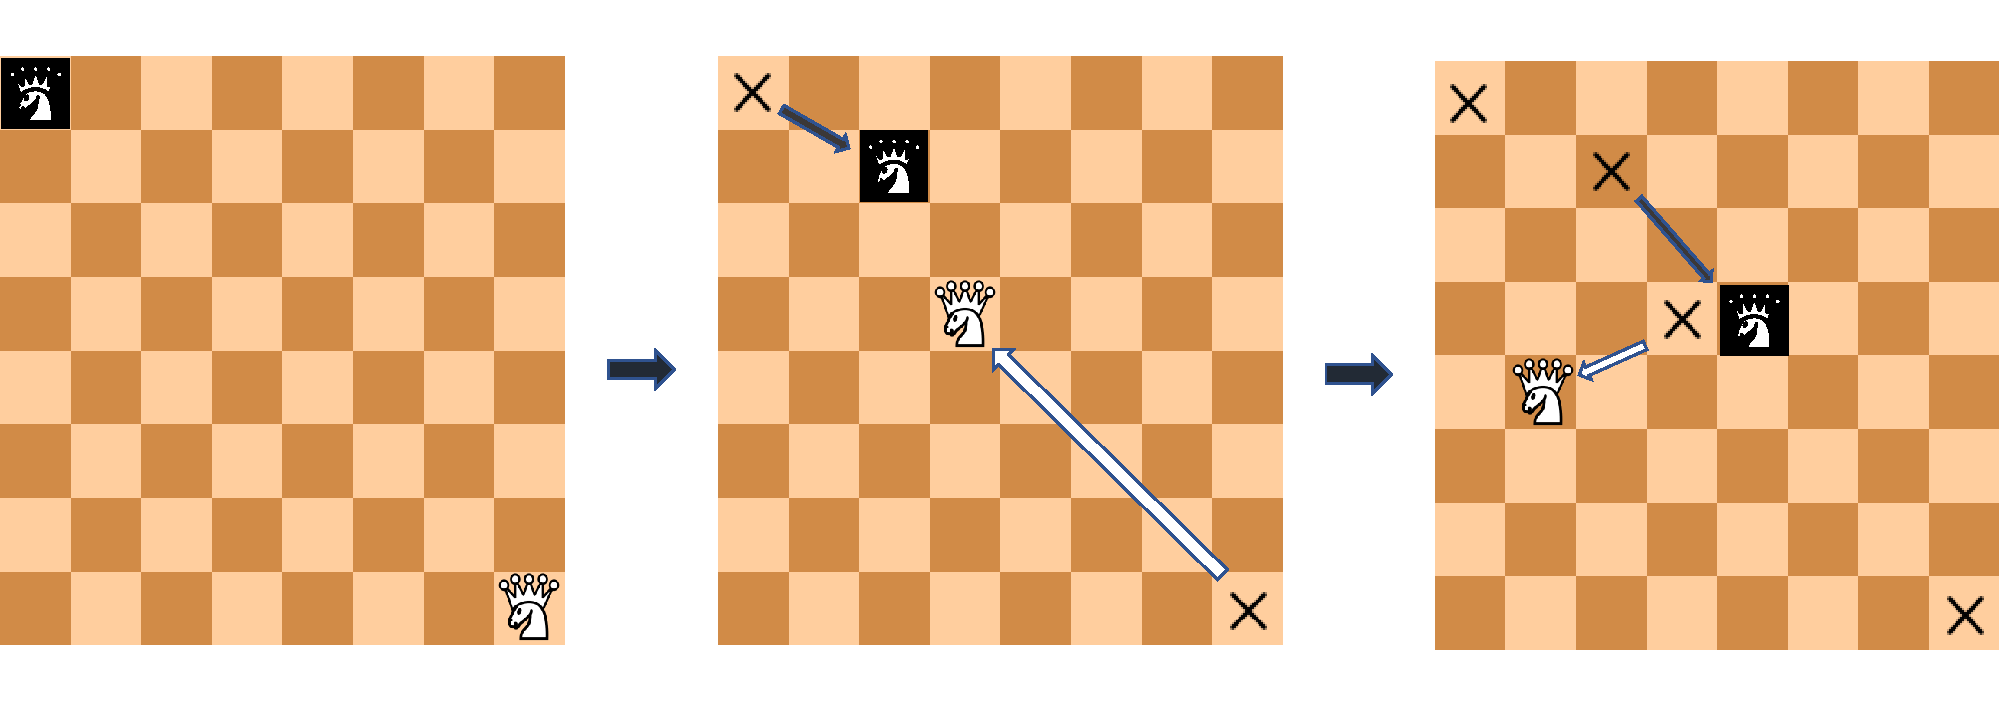
\includegraphics[width=0.8\textwidth]{super.pdf}
    \caption[rules-super]{%
        超级皇后对战游戏规则——超级状态%
      }
    \label{fig:super}
\end{figure}
骑士状态下,不论是~alpha-beta~剪枝还是蒙特卡洛树搜索进行模拟速度都相对较快,因此在自我对弈阶段的落子速度也很快,但由于博弈树复杂度较低,启发式搜索算法的效果可能会好于基于蒙特卡洛树搜索的~AlphaZero~框架,因为其可以在较短时间内较小深度下搜索大部分个博弈树,其局部最优解更靠近全局最优解。
而超级状态下每回合平均合法移动数目相对较多,搜索代价较大,在同等时间限制下更加适合深度强化学习~AlphaZero~训练出的模型。

\section{基准玩家设计}
我们总共实现了4个AI玩家:随机玩家(Random Player),贪婪玩家(Greedy Player),alpha-beta剪枝玩家, AlphaZero型玩家。前三个玩家将作为基准玩家(baseline player)。
\paragraph{随机玩家}
随机玩家,顾名思义,即为其每步动作都基于当前可行走法进行随机选择。在每一回合开始,随机玩家先输出自己的可选动作列表,并在此列表中随机选择一个作为自己在这一回合的动作。如图~\ref{fig:super},白色圆点代表白色方可行动作,随机玩家将从这些白色圆点里选择。
\begin{figure}[htb]
    \centering
    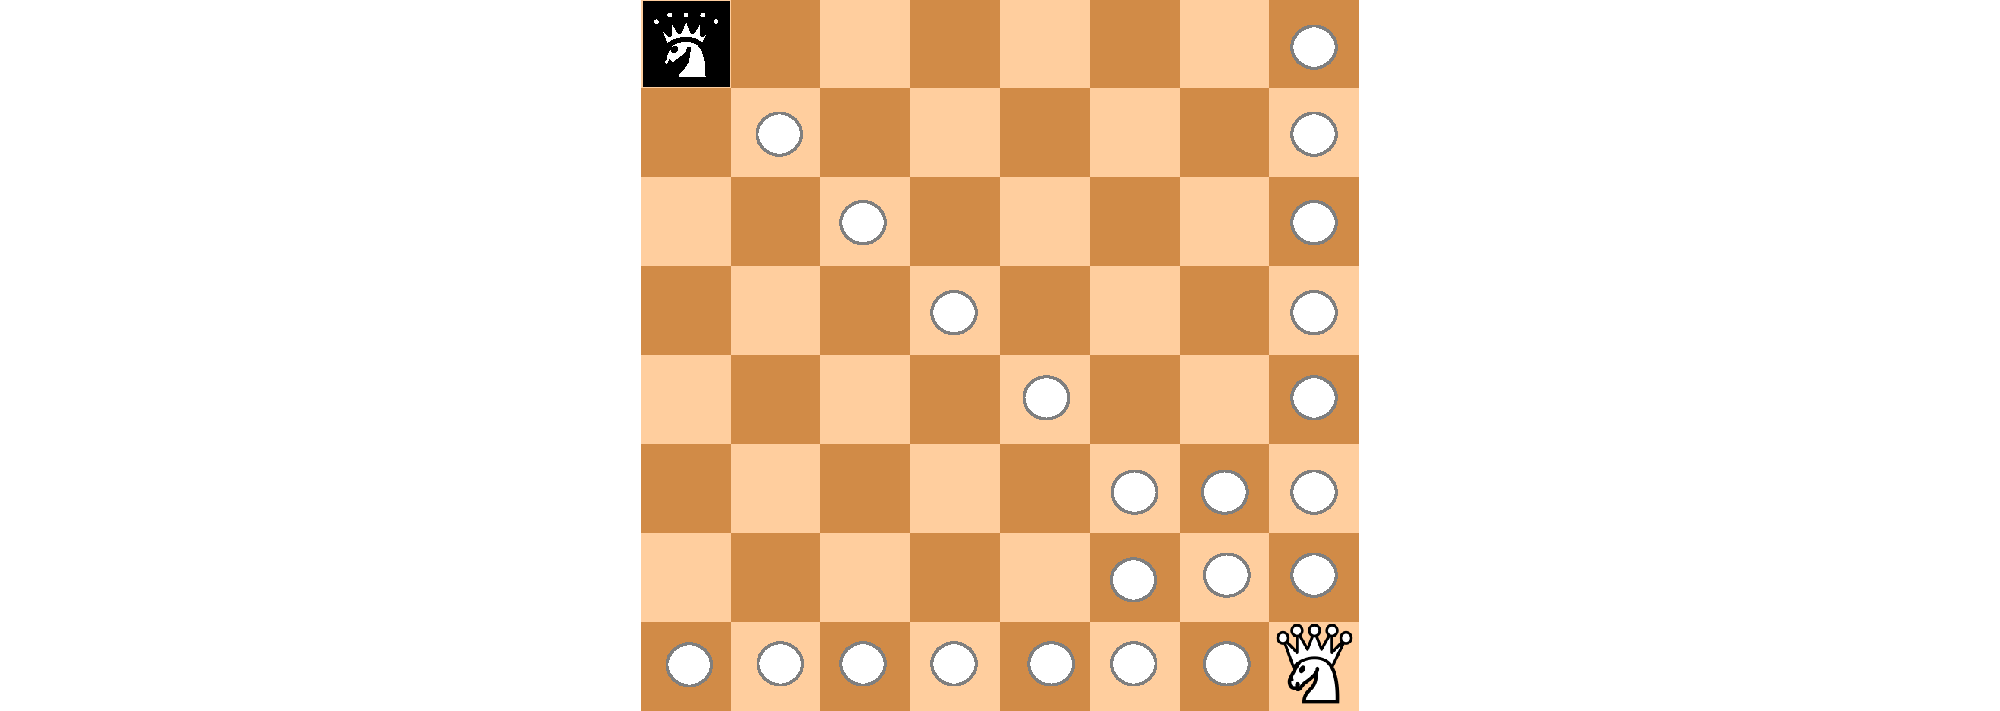
\includegraphics[width=1\textwidth]{rp.pdf}
    \caption[rp]{%
        随机玩家在白色圆点中任选%
      }
    \label{fig:super}
\end{figure}
\paragraph{贪婪玩家}
贪婪玩家采取的是贪心算法~\cite{introAlgo}。这是寻找问题最优解的常见方法,在问题的每个步骤都采取贪心原则,即选取当前状态下最好的选择(局部最优解)。因此我们需要一个评价函数来衡量棋盘状态对于玩家的好坏,经过比较与实验,定义评价函数如下:
\begin{equation}
    Score(\text{player}) = Count(LegalMoves(\text{player})) - Count(LegalMoves(\text{opponent}))
\end{equation}
在某一回合,当前选手有若干个合法行动可选,我们需要评估出其在遍历每一个行动后棋盘盘面的好坏。评估盘面好坏使用上述评估函数,玩家在一步之后的合法行动数量减去对手合法行动数量的值越大,说明该步是当前玩家的最优解,将遍历后得到的分数分数进行排序选择最大值对应的行动即可。
假设当前是黑色方回合,局势如图~\ref{fig:gp1}。
\begin{figure}[htb]
    \centering
    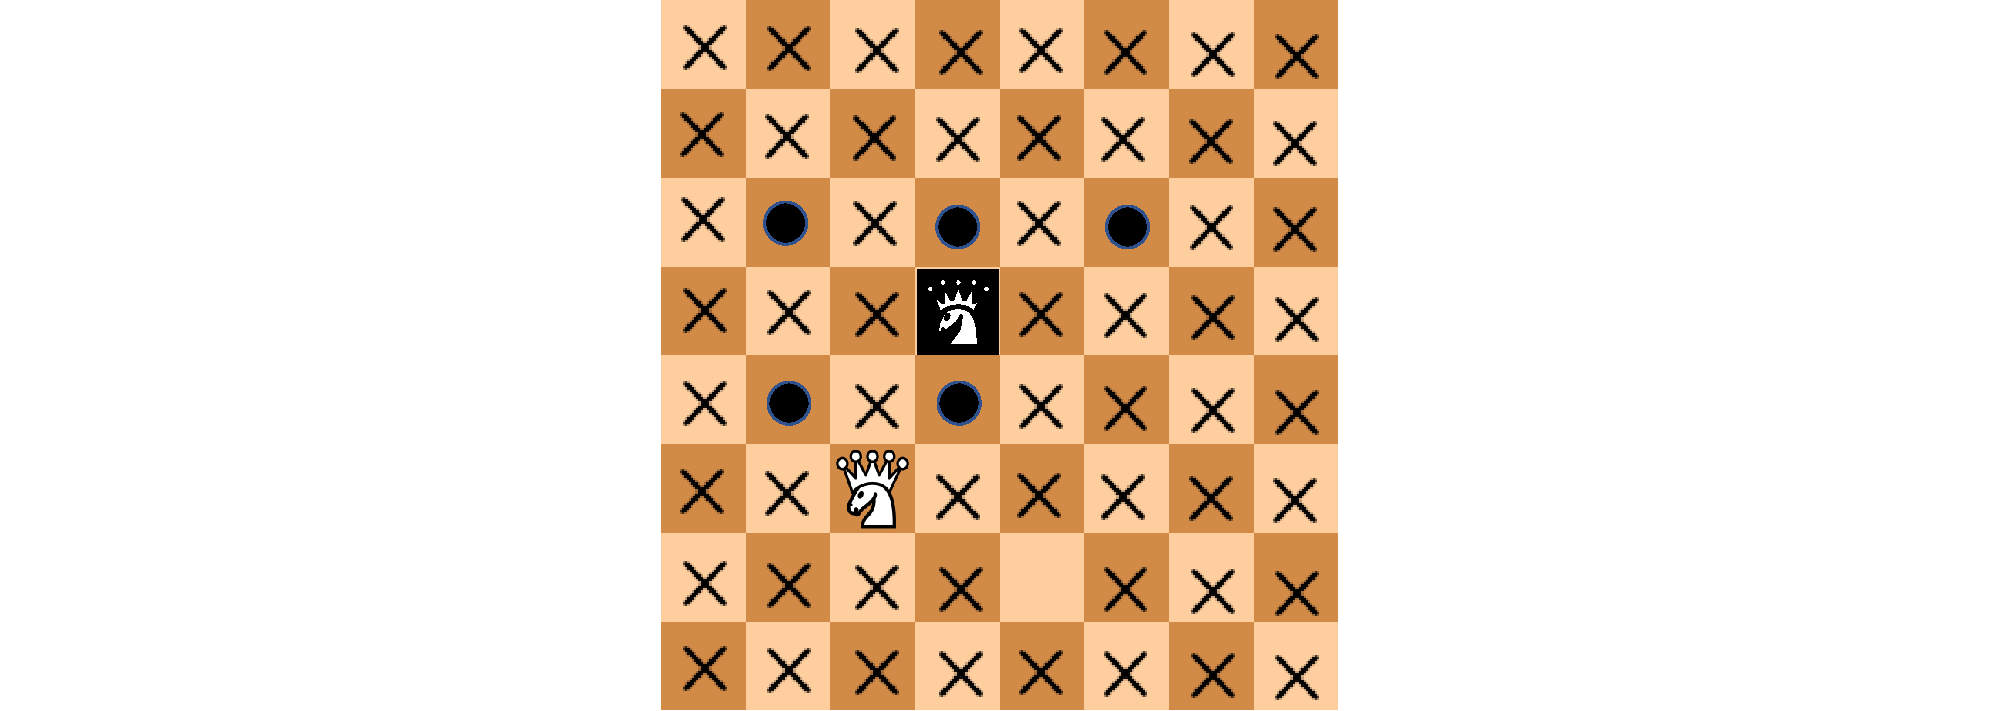
\includegraphics[width=1\textwidth]{gp1.pdf}
    \caption[gp1]{%
        黑色圆点代表当前黑色超级皇后合法行动%
      }
    \label{fig:gp1}
\end{figure}
黑色圆点代表其合法行动落点,其有五个合法落子位置可选,我们分别计算假设黑色方落到各个位置后的分数如图~\ref{fig:gp2}:
\begin{figure}[htb]
    \centering
    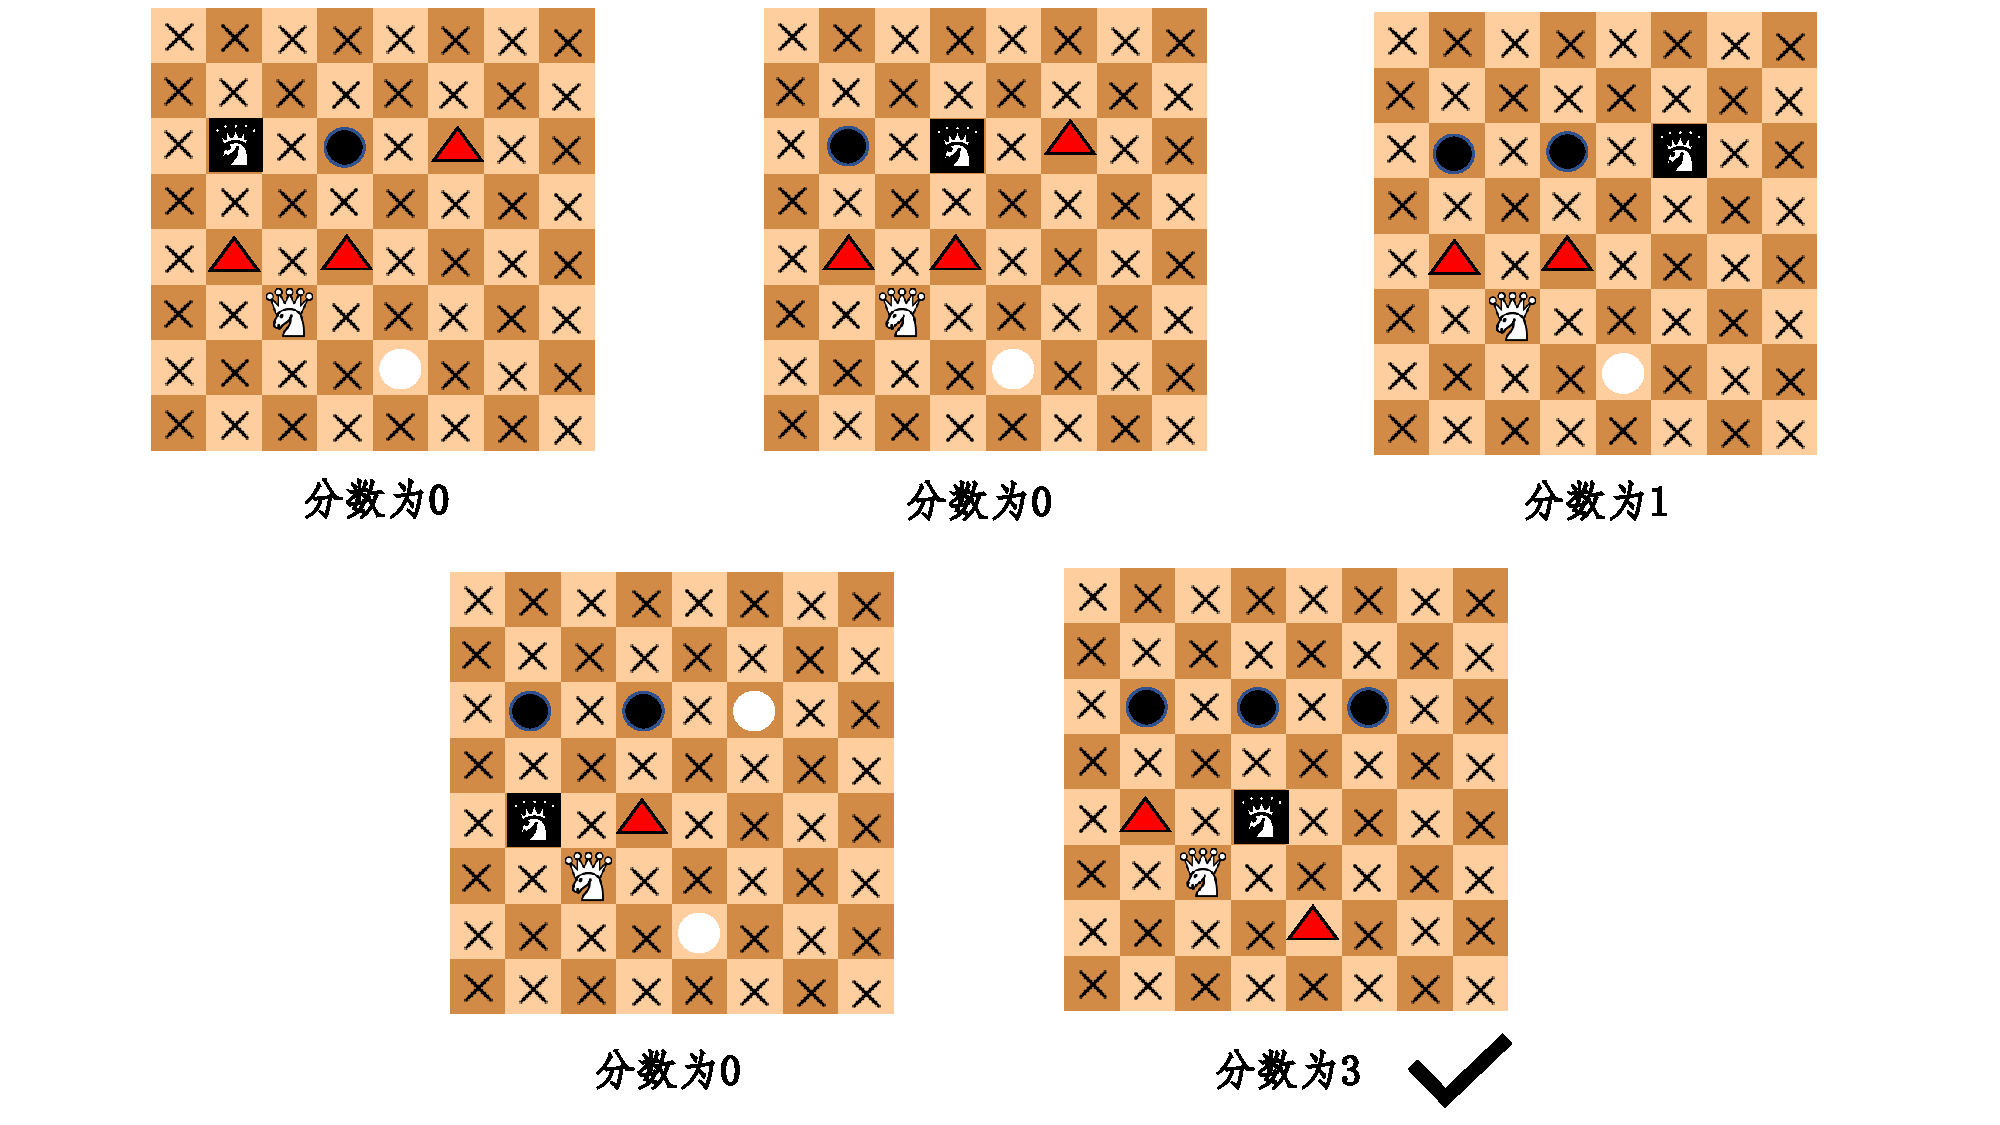
\includegraphics[width=1\textwidth]{gp2.pdf}
    \caption[gp2]{%
        分数计算与走法选择%
      }
    \label{fig:gp2}
\end{figure}
黑色圆点代表仅属于黑色超级皇后的合法行动,白色圆点代表仅属于白色超级皇后的合法行动,红色三角形代表双方共享的合法行动,根据分数计算结果,选择分数为3的走法。
\paragraph{alpha-beta剪枝玩家}
在剪枝搜索过程中,我们仍使用在贪婪玩家部分中定义的评价函数更新叶节点的值。考虑
到博弈树过深引起的搜索时间代价~\cite{sstextbook},alpha-beta剪枝玩家的深度设置为4。
初始$\alpha$值设置为~$-99$,$\beta$值设置为~$99$。假设当前是黑色方回合,局势仍然如图~\ref{fig:gp1}。搜索与剪枝过程可表现为图~\ref{fig:abpde}。
\begin{figure}[htb]
    \centering
    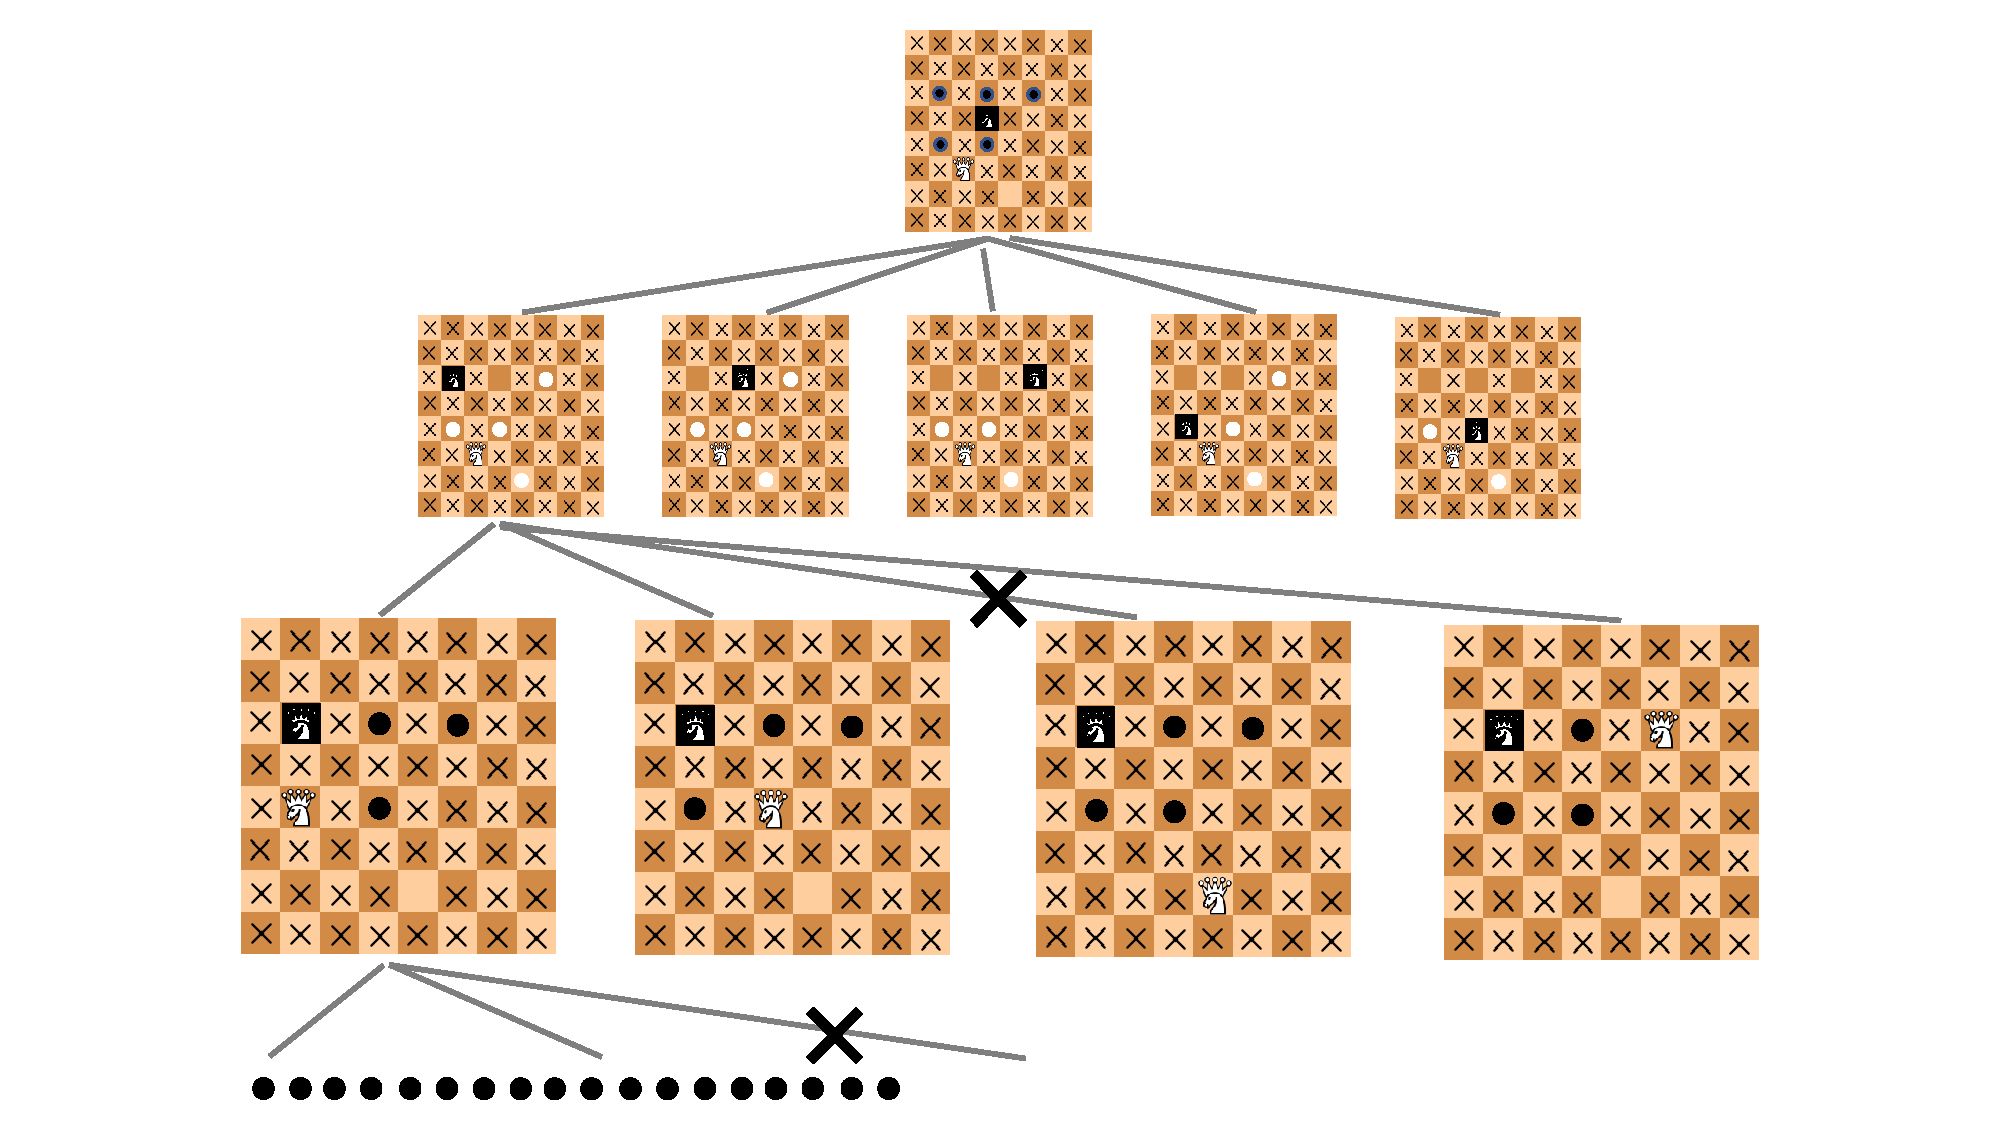
\includegraphics[width=1\textwidth]{abp_design.pdf}
    \caption[abpde]{%
        超级皇后对战搜索与剪枝%
      }
    \label{fig:abpde}
\end{figure}

\section{深度强化学习玩家设计}
超级皇后对战是一款全新游戏,它没有人类专家棋谱与对弈棋局数据库供我们使用监督学习训练。这也意味着我们需要从白板状态训练出一个足够胜过基准玩家的AI玩家,因此我们将参考~AlphaGo Zero~与~AlphaZero~的框架,使用基于单一神经网络并纳入蒙特卡洛树搜索的策略迭代(policy iteration)对超级皇后对战进行训练~\cite{Silver1140,Silver2017,Silver2016}。

相比于基准玩家,强化学习玩家只采取棋盘上的棋子与空位死位作为输入特征,不需要人为设计分数函数与杀棋特征。考虑到棋盘特征是二维的数据,且在强化学习过程中的自我对弈(self play)会生成大量数据,因此非常适合使用卷积神经网络对棋面局势进行评估以及对走棋动作进行选择~\cite{Silver2016}。

\subsection{数据生成过程}
在自我对弈过程中,使用前一轮训练出的网络指导蒙特卡洛树进行对弈。对于每一局的每个回合$t$下的棋面局势$board_{t}$,蒙特卡洛树搜索模拟过程产生下一步走棋策略(概率分布)$\pi_{t}$并生成数据对$(board_{t},\pi_{t})$。
在每局结束时,对弈双方得到奖励为$v$(胜者为1,负者为~-1),将此奖励值作为分类标签贴到在这一次对弈生成的数据对中产生$(board_{t},\pi_{t},v_{t})$,其中$v_{t}=\pm v$,正负符号当前棋局下棋方决定。
在训练时,$board_{t}$为输入网络的样本,棋局特征将从其二维结构中提取。$(\pi_{t},v_{t})$为$board_{t}$的标签,网络输出对应为$(p,v)$,拟合标签。
\subsection{策略网络与值网络}
在原版的~AlphaGo~模型~\cite{Silver2016}中,使用了两个网络,分别是策略网络(policy network)与值网络(value network),对应策略迭代算法中的策略函数与值函数。策略网络输出下一步动作的概率分布,即给出选择哪种动作的可能性更大;值网络评估当前棋面局势好坏,预测可能的获胜者。
但是~AlphaGo~的策略网络在一开始使用监督学习训练专家棋谱,再使用强化学习算法如策略梯度方法(policy gradient~\cite{silver2014deterministic}),而其值网络从策略网络的自我对弈过程中学习并预测胜者。如前面所述,我们没有专家棋谱进行监督学习,因此参考~AlphaGo Zero~与~AlphaZero~使用单一网络输出概率分布与预测值是不错的选择。
我们采取以下两种不同结构的神经网络分别训练:
\paragraph{经典卷积神经网络}
经典卷积神经网络结构较为简单,层数较少,网络的参数量也较少,但比较适合提取$8\times8$的棋盘特征。其结构如图~\ref{fig:cnn}所示:
(1)2D卷积层(适用图像的空间卷积),该层创建的卷积核对层输入进行卷积以生成输出张量,需要边缘填充(padding)操作填充输入以使输出具有与原始输入相同的长度,其输出空间的维度为512;
(2)批量标准化层~\cite{batchnorm},在当前批次数据中标准化前面卷积层的激活项,特征轴设置为3;
(3)使用整流线性单位函数(Rectified Linear Unit, ReLU)~\cite{xu2015empirical}激活一次,减少计算结果;
(4)以上三步再重复3次,在后两次中不需要进行padding操作;
(5)Flatten层将输入展平;
(6)全连接层,其输出空间维度为1024,在进行标准化后使用ReLU函数激活并使用丢弃(Dropout)~\cite{srivastava2014dropout}防止过拟合;
(7)全连接层,其输出空间维度为512,在进行标准化后使用ReLU函数激活并使用丢弃(Dropout)防止过拟合;
(8)使用Softmax激活函数\footnote{归一化指数函数,是逻辑函数的一种推广。}的全连接层输出维度为动作空间大小(action size)的概率值$p$;
(9)使用双曲正切激活函数(tanh)的全连接层输出维度为1的奖励值(预测胜者)$v$;
\begin{figure}[H]
    \centering
    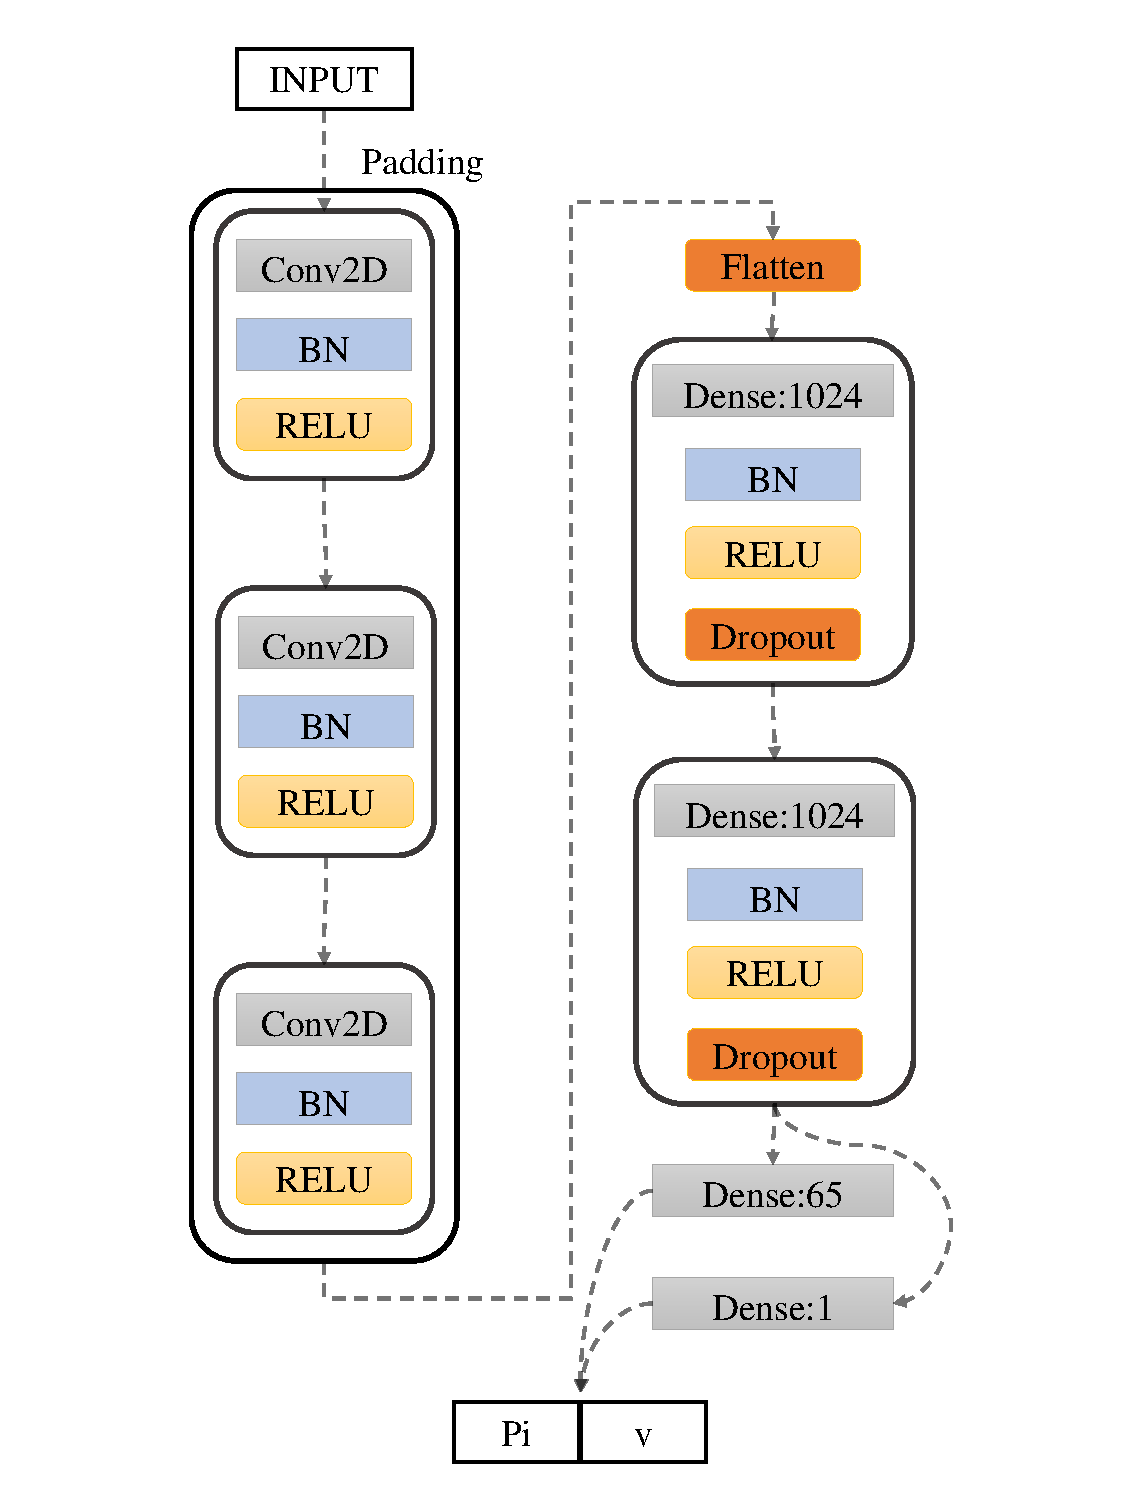
\includegraphics[width=0.9\textwidth]{classic.pdf}
    \caption[cnn]{%
    经典卷积神经网络%
      }
    \label{fig:cnn}
\end{figure}
\paragraph{深度残差网络}
深度残差网络是具有重要地位的经典计算机模型~\cite{resnet}。对于我们超级皇后的棋局而言,经典卷积神经网络不够深,即便其能较好地适应$8\times8$的棋盘特征,但是在训练大量对局数据中仍有可能出现性能瓶颈。
因此我们需要考虑加深网络层数,例如说在经典卷积神经网络中继续增加卷积层。但是更深的网络性能通过实验证明会出现退化问题:深度增加时,损失(loss)减少但准确度下降~\cite{resnet,he2016identity}。
考虑到代价与实际需求,深度残差网络是一个较为合适的选择~\cite{resnet}。其核心结构为设计了短路连接(shortcut connection)使若干卷积层的集合能学习到残差带来的新特征,如图~\ref{fig:resunit}所示:
\begin{figure}[H]
    \centering
    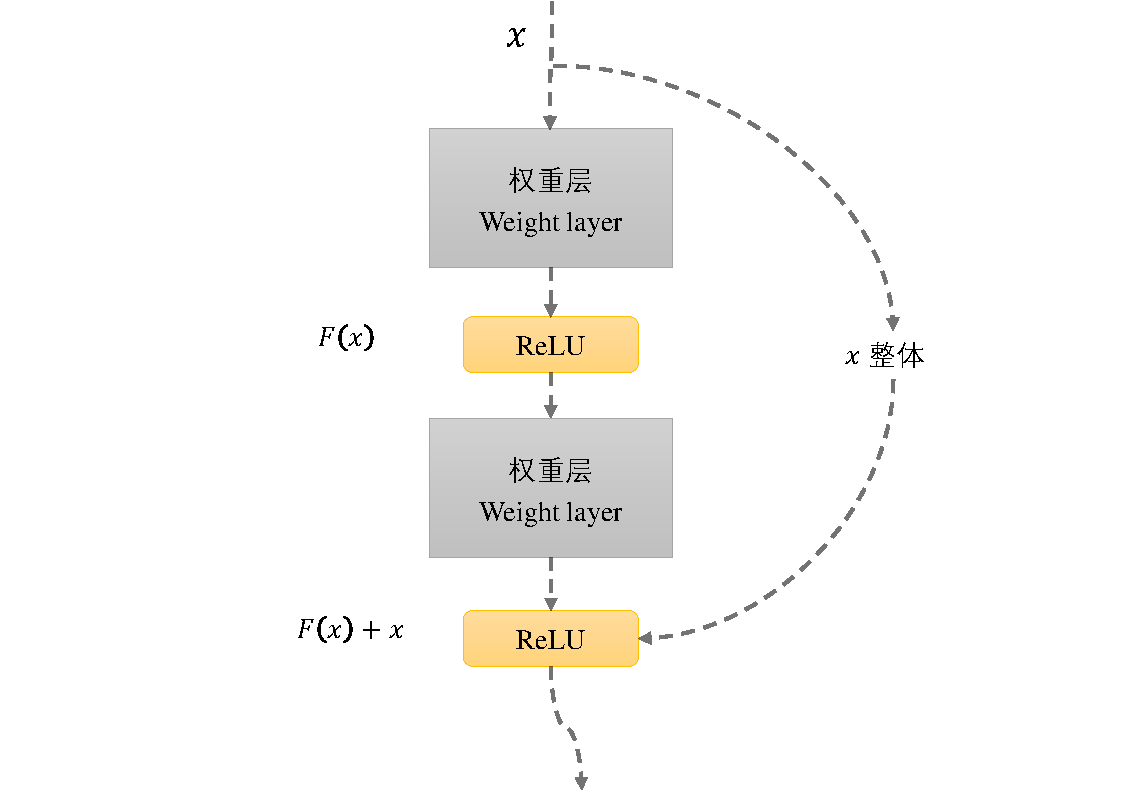
\includegraphics[width=0.7\textwidth]{resnetblcok.pdf}
    \caption[resunit]{%
    残差学习单元~\cite{resnet}%
      }
    \label{fig:resunit}
\end{figure}
对于如图的若干卷积层构成的堆积层,输入为$x$时其学习到的特征我们用$H(x)$表示,其残差可以表示为$F(x)=H(x)-x$。要学习到残差$F(x)$,其原始学习特征为$F(x)+x$。残差学习相比原始特征直接学习更容易,也会使得图中残差结构单元在输入特征基础上学习到新的特征,从而拥有更好的性能。
在训练超级皇后对战时,深度残差网络结构如图~\ref{fig:res},输入层的reshape方式以及Flatten层后的结构与经典卷积神经网络一致,图中$/S$代表步长(stride),$F$代表滤波器(filter)数量。
\begin{figure}[H]
    \centering
    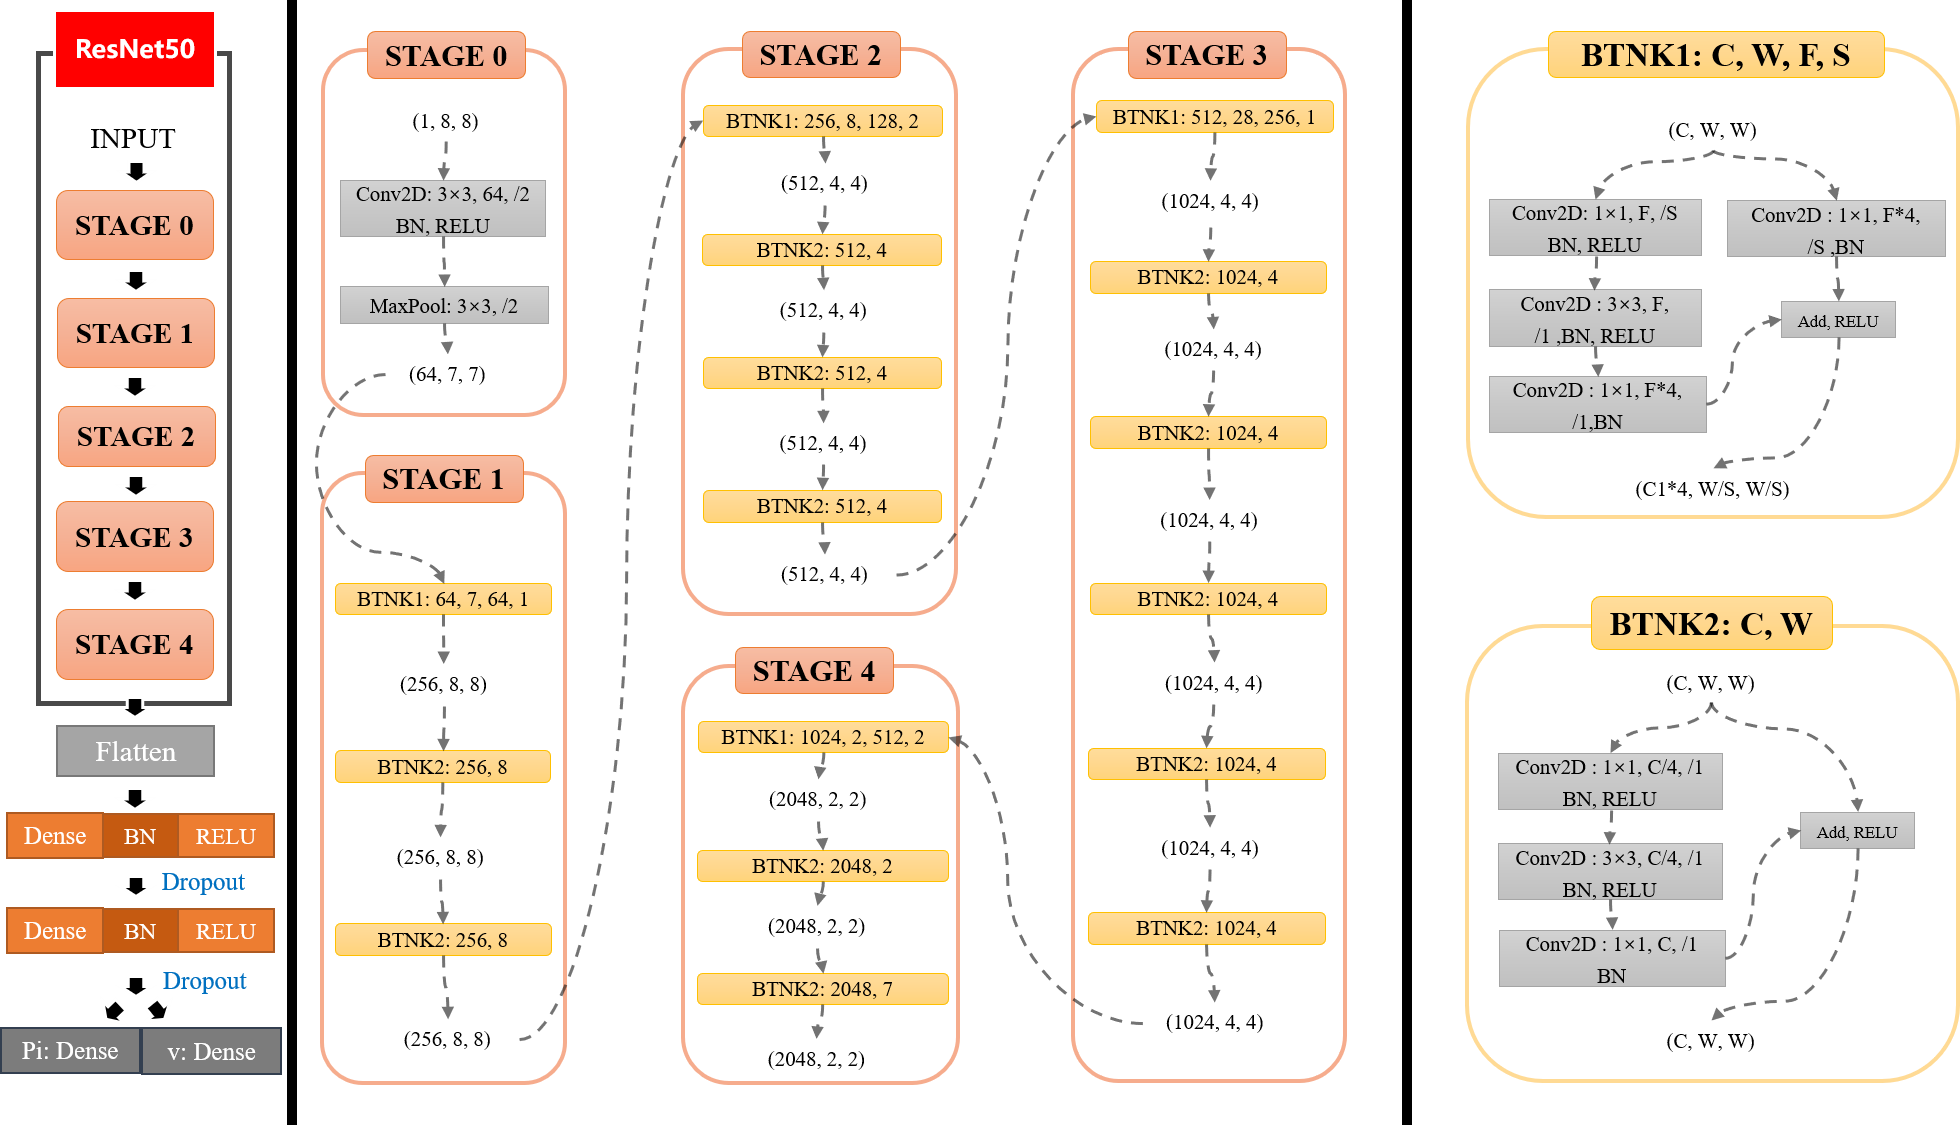
\includegraphics[width=1\textwidth]{resnet.pdf}
    \caption[res]{%
    深度残差网络:以ResNet50为基础~\cite{resnet}%
      }
    \label{fig:res}
\end{figure}
深度残差网络可以更好地学习到棋盘特征,并且棋盘越大(如$12\times12$,$16\times16$),其学习效果越好。但是超级皇后对战的局势并没有特别复杂,因此使用深度残差网络也有可能导致模型过拟合或欠拟合。

针对以上神经网络,损失函数我们仿照~\cite{Silver2017}中的结构,该结构结合了均方误差(mean-square error, MSE)与类别交叉熵,能够较好地最小化$v$与标签$v_{t}$的误差,最大化$p$与$\pi_{t}$的相似度。为了防止过拟合,我们在网络中添加dropout层与l2正则化。
\begin{equation}
    \text{loss} = (v_{t}-v)^{2} - \pi^{T}\log(p)
\end{equation}
\subsection{策略迭代应用}
上述两个神经网络使用策略迭代算法在超级皇后的自我对弈中进行训练,我们用$f$表示神经网络。对于每个棋面状态,使用前一轮训练得到的函数(也就是神经网络$f$)对蒙特卡洛树搜索进行指导。
蒙特卡洛树搜索(MCTS)可以被看作是策略迭代算法中的策略提升(Policy Improvement):MCTS会输出每一步动作的概率分布$\pi$,该概率分布被称为搜索概率~\cite{silver2009reinforcement}。搜索概率比神经网络输出的概率分布$p$更好,可以选出更好的走棋动作。
而在超级皇后自我对弈过程中,使用基于神经网络输出,经过蒙特卡洛树搜索提升的策略函数$\pi$进行动作选择并最终决出胜负生成新的训练样本,可以被看作是策略迭代算法中的策略评估(Policy Evaluation):评估当前局势并预测获胜概率。
在蒙特卡洛树搜索结束后,使用新对弈样本更新神经网络参数,使其输出$(p,v)=f(board)$更加靠近MCTS得到的搜索概率与获胜方的策略。
更新后的神经网络与更新前的神经网络各自指导MCTS进行若干局对弈,若更新后的神经网络胜率超过$60\%$,则其将在下一轮训练中使用新的神经网络进行自我对弈并继续指导MCTS,继续增强走棋能力。否则继续使用更新前的神经网络。

在进行搜索模拟时,从代表当前棋盘局面的搜索树根节点$s$开始,每个节点$o$会被赋予访问次数$N(o,s,a)$,奖励值$Q(o,s,a)$与先验概率$P(o,s,a)$,$a$代表走棋动作,过程如下:

(1) 选择(Selection):从根节点$s$开始,通过选择使置信上界最大的动作$a_{o} = argmax(UCT(o,s,a)) = argmax(Q(o,s,a) + U(o,s,a))$进行搜索直到叶子节点,其中
\begin{equation}
    U(o,s,a) = cP(o,s,a)\frac{\sqrt{N(\prime,s,a)}}{1+N(o,s,a)}
\end{equation}
常数$c$平衡高胜率与低访问次数的关系,决定探索力度~\cite{rosin2011multi}。
(2) 扩展(Expansion):叶子节点访问次数达到一个阈值时,创建新的子节点$s^{\prime}$进行选择。使用神经网络产生的先验概率$P(s^{\prime},\prime)$和评估值$v(s^{\prime})$进行选择。

(3) 反向传播(Backpropagation):更新叶子节点路径上所有边与节点的访问次数与奖励值如下,并回到步骤1~\cite{segal2010scalability}。
\begin{equation}
    \begin{aligned}
    Q(o,s,a) &= \frac{\sum^{s^{\prime}|s,a\rightarrow s^{\prime}}v(s^{\prime})}{1+N(o,s,a)} \\
    N(o,s,a) &+= 1 
    \end{aligned}
\end{equation}
多次进行搜索模拟后最终得到搜索概率$\pi$,可以使用该搜索概率抽样走棋动作并完成此回合落子。至此,我们使用强化学习参考AlphaZero框架对超级皇后对战进行训练的过程如图~\ref{fig:az}所示。
\begin{figure}[H]
    \centering
    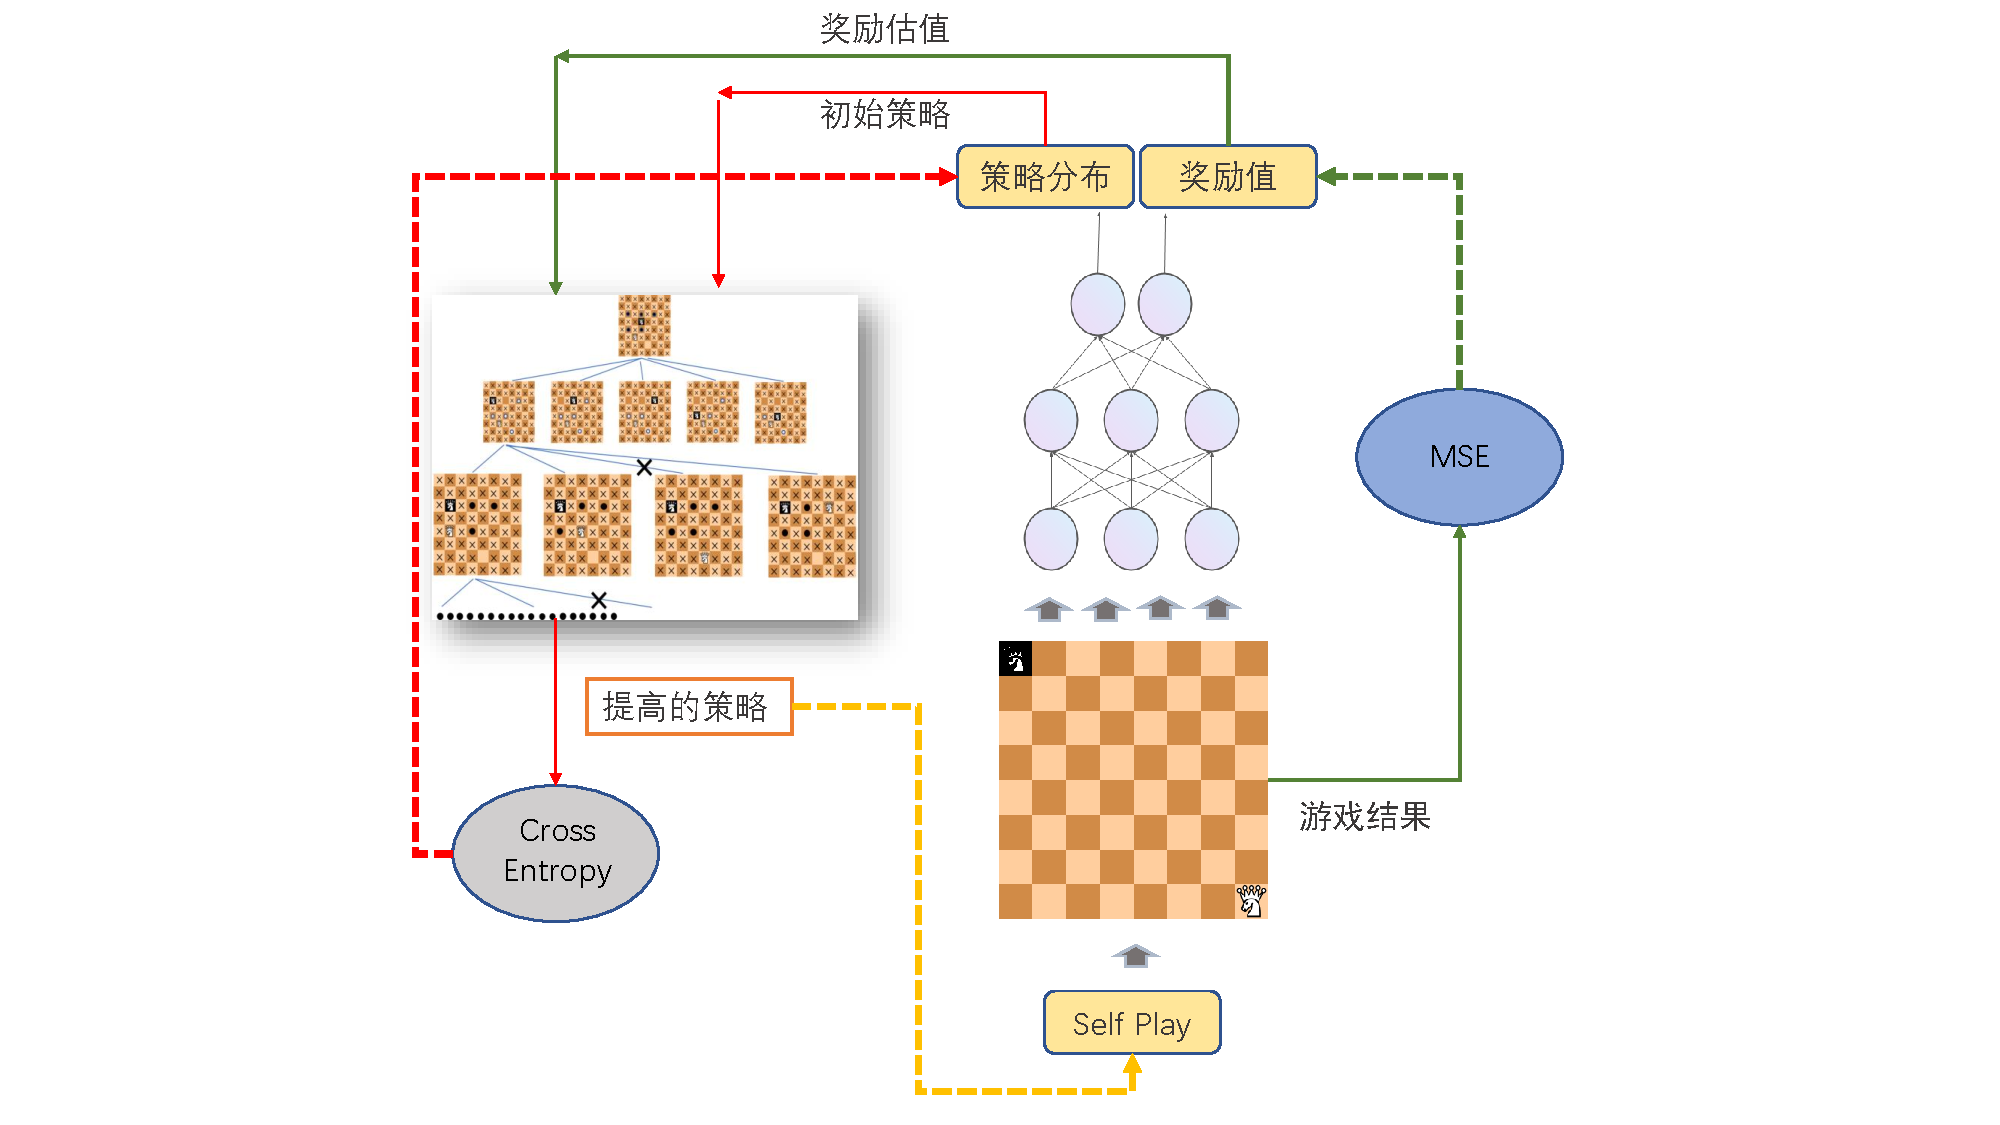
\includegraphics[width=1\textwidth]{alphazero.pdf}
    \caption[az]{%
    以AlphaZero为框架的强化学习玩家~\cite{Silver2017}%
      }
    \label{fig:az}
\end{figure}


